\section{Tia Nur Candida - 1174086}
\subsection{Teori}
\begin{enumerate}
\item Definisi Kecerdasan Buatan \\
Kecerdasan Buatan adalah suatu ilmu yang mempelajari bagaimana cara komputer melakukan sesuatu seperti yang dilakukan oleh manusia. Secara sederhana AI adalah teknik dan ilmu untuk membangun atau membuat suatu mesin menjadi cerdas, terutama pada program komputer. Kecerdasan yang dimaksud yaitu seperti yang dimiliki oleh manusia namun pada mesin akan dibuat cepat dan tepat atau akurat.

\item Sejarah Kecerdasan Buatan \\
Sejarah kecerdasan buatan dimulai pada zaman kuno. Benih kecerdasan buatan modern ditanamkan oleh filusuf klasik dengan berusaha menggambarkan proses berpikir manusia. Karya tersebut memuncak pada penemuan komputer digital yang di program pada tahun 1940 an, dimana terdapat sebuah mesin yang didasarkan pada esensi abstrak penalaran matematika. 
Istilah kecerdasan buatan pertama kali dikemukaan pada tahun 1956 di Konferensi Darthmouth yang kemudian sejak saat itu kecerdasan buatan terus berkembang.

\begin{itemize}
\item Masa Persiapan AI (1943-1956)\\
Pada tahun 1943, Warren McCulloch dan Walter Pitt mengemukakan tiga hal : pengetahuan fisiologi dasar dan fungsi sel syaraf dalam otak, analisa formal tentang logika proposisi, dan teori komputasi Turing. Mereka berhasil membuat suatu model sel syaraf tiruan dimana setiap sel syaraf digambarkan sebagai ‘on’ dan ‘off’. Mereka menunjukkan bahwa setiap fungsi dapat dihitung dengan suatu jaringan sel syaraf dan bahwa semua hubungan logis dapat diimplementasikan dengan struktur jaringan yang sederhana.
Pada tahun 1950, Nobert Wiener membuat penelitian mengenai prinsip-prinsip teori feedback. Contoh yang terkenal adalah thermostat. Penemuan ini juga merupakan awal dari perkembangan AI.

Pada tahun 1956, John McCarthy meyakinkan Minsky, Claude Shannon dan Nathaniel Rochester untuk membantunya melakukan penelitian dalam bidan Otomata, Jaringan Syaraf dan pembelajaran intelijensia. Mereka mengerjakan proyek ini selama 2 bulan di Dartsmouth. Hasilnya adalah program yang mampu berpikir non-numerik dan menyelesaikan masalah pemikiran, yang dinamakan Principia Mathematica. Hal ini menjadikan McCarthy disebut sebagai bapak kecerdasan buatan.


\item Awal perkembangan AI (1952-1969)\\
Kecerdasan buatan banyak mengalami kesuksesan pada tahun pertama. 
Pada tahun 1958, McCarthy di MIT AI Lab Memo No.1 mendefinisikan bahasa pemrograman tingkat tinggi yaiyu LISP, yang sekarang mendominasi pembuatan program-pogram kecerdasan buatan. Kemudian, McCarthy membuat program yang dinamakan Programs with Common Sense. Di dalam program tersebut, dibuat rancangan untuk menggunakan pengetahuan dalam mencari solusi.
Pada tahun 1959, Nathaniel Rochester dari IBM dan mahasiswa-mahasiswanya mengeluarkan program kecerdasan buatan yaitu Geometry Theorm Prover. Program ini dapat mengeluarkan suatu teorema menggunakan aksioma-aksioma yang ada.
Pada tahun 1963, program yang dibuat James Slagle mampu menyelesaikan masalah integral tertutup untuk mata kuliah Kalkulus.
Pada tahun 1986, program analogi buatan Tom Evan menyelesaikan masalah analogi geometris yang ada pada tes IQ.

\item Perkembangan kecerdasan buatan melambat (1966-1974)
Banyak masalah yang perlu di selesaikan oleh kecerdasan buatan dan baru sedikit program yang keluar menyebabkan melambat.

\item Kecerdasan buatan menjadi sebuah industri ( 1980 - 1988 )\\
Industrialisasi kecerdasan buatan diawali dengan ditemukannya sistem pakar yang dinamakan R1 yang mampu mengkonfigurasi system-sistem computer baru. Program tersebut mulai dioperasikan di Digital Equipment Corporation (DEC), McDermott, pada tahun 1982.
Pada tahun 1986, R1 telah berhasil menghemat US Dolar 40 juta per tahun.
Pada tahun 1988, kelompok kecerdasan buatan di DEC menjalankan 40 sistem pakar. Hampir semua perusahaan besar di USA mempunyai divisi AI. Sehingga perusahaan yang sejak tahun 1982 hanya menghasilkan beberapa juta US dolar per tahun meningkat menjadi 2 milyar US dolar per tahun pada tahun 1988.

\item Kembalinya Jaringan Syaraf Tiruan ( 1986 - Sekarang )\\
Meskipun bidang ilmu computer menolak jaringan syaraf tiruan setelah diterbitkannya buku “Perceptrons” karangan Minsky dan Papert, tetapi para ilmuwan masih mempelajari bidang ilmu tersebut dari sudut pandang yang lain yaitu fisika. Para ahli fisika seperti Hopfield (1982) menggunakan teknik-teknik mekanika statistika untuk menganalisa sifat-sifat pentimpanan dan optimasi pada jaringan syaraf. Para ahli psikologi, David Rumelhart dan Geoff Hinton, melanjutkan penelitian mengenai model jaringan syaraf tiruan pada memori.
Pada tahun 1985-an setidaknya empat kelompok riset menemukan kembali algoritma belajar propagasi balik (Black-Propagation Learning). Algoritma ini berhasil diimplementasikan ke dalam bidang ilmu computer dan psikologi.

\end{itemize}
\item Definisi Supervised Learning \\
Merupakan tipe Machine Learning dimana model ini menyediakan training data berlabel. Supervised learning merupakan suatu pembelajaran yang terawasi dimana jika output yang diharapkan telah diketahui sebelumnya.  Supervised Learning adalah tipe learning di mana kita mempunyai variable input dan variable output, dan menggunakan satu algoritma atau lebih untuk mempelajari fungsi pemetaan dari input ke output. Goal-nya adalah untuk memperkirakan fungsi pemetaannya, sehingga ketika kita mempunya input baru, kita dapat memprediksi output untuk input tersebut.

\item Klasifikasi
\begin{itemize}
\item Logistic regression
\item K-nearest neighbors
\item Support vector machine (SVM)
\item Naive Bayes
\item Decision tree classification
\item Random forest classification
\end{itemize}

\item Regresi \\
Regresi adalah suatu metode analisis statistik yang digunakan untuk melihat pengaruh antara dua atau lebih banyak variabel. Hubungan variabel tersebut bersifat fungsional yang diwujudkan dalam suatu model matematis.

\item Unsupervised Learning \\
Unsupervised Learning adalah tipe learning di mana kita hanya mempunyai data masukan (input data) tetapi tidak ada output variable yang berhubungan.\\
Goal dari unsupervised learning adalah untuk memodelkan struktur dasar atau distribusi dalam data dengan tujuan untuk mempelajari data lebih jauh lagi, dengan kata lain, adalah menyimpulkan fungsi yang mendeskripsikan atau menjelaskan data.

\item Dataset \\
Dataset adalah objek yang merepresentasikan data dan relasinya di memory. Strukturnya mirip dengan data di database. Dataset berisi koleksi dari datatable dan datarelation.
\item Training Set \\
Training set adalah bagian dataset yang kita latih untuk membuat prediksi atau menjalankan fungsi dari sebuah algoritma ML lainnya sesuai tujuannya masing-masing. Kita memberikan petunjuk melalui algoritma agar mesin yang kita latih bisa mencari korelasinya sendiri.
\item Test Set \\
Test set adalah bagian dataset yang kita tes untuk melihat keakuratannya, atau dengan kata lain melihat performanya.

\end{enumerate}
\subsection{Praktek}
\begin{enumerate}
	\item Instalasi Library scikit dari anaconda, mencoba kompilasi dan uji coba ambil contoh kode dan lihat variabel explorer
	\hfill\break
	\begin{figure}[H]
		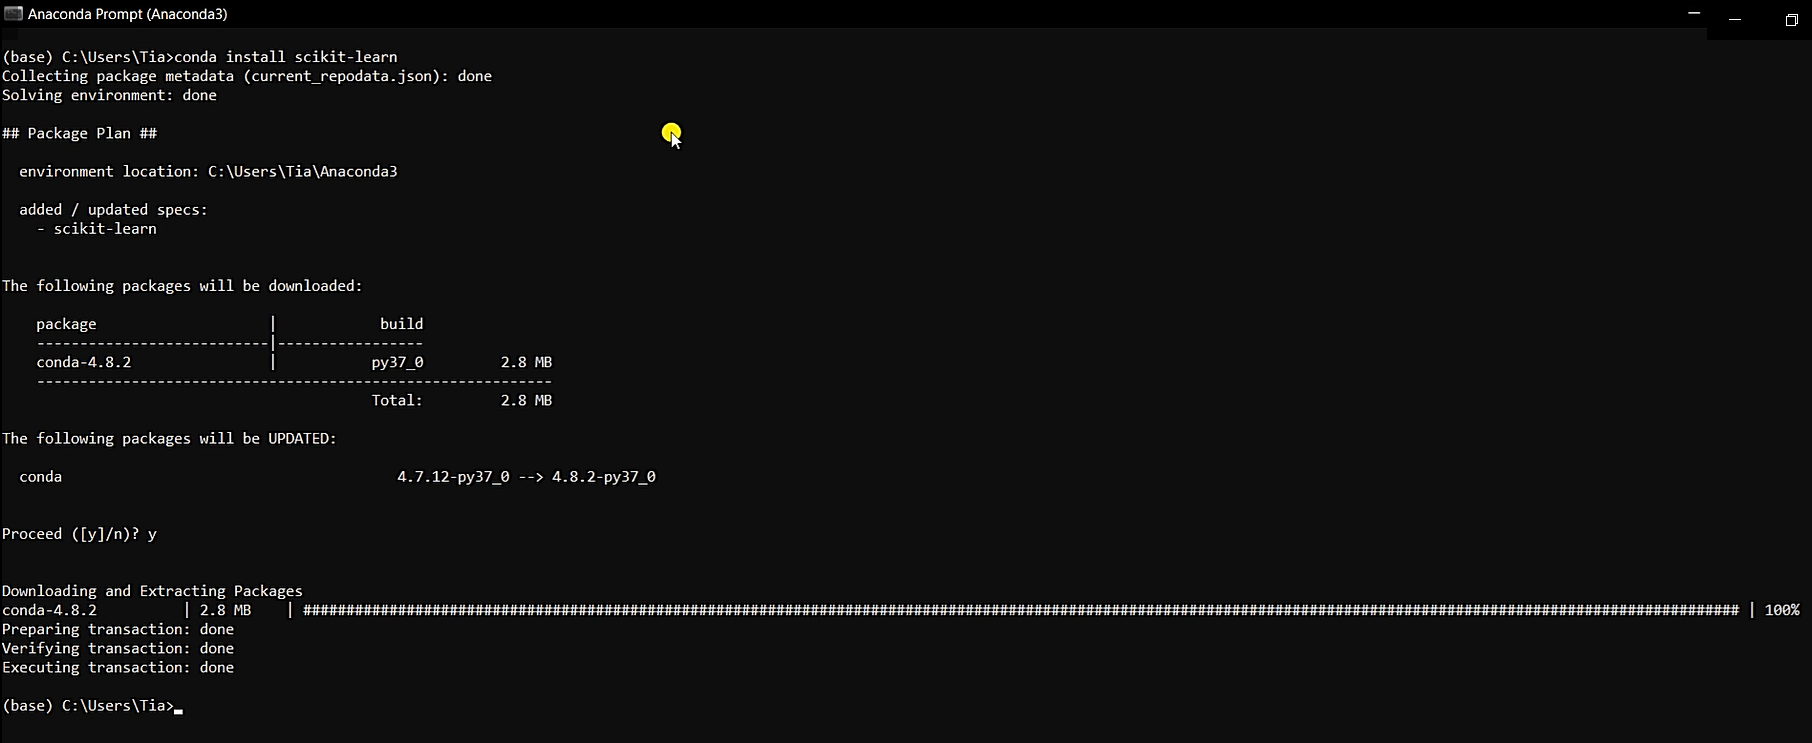
\includegraphics[width=4cm]{figures/1174086/1/installasi.PNG}
		\centering
		\caption{Instalasi Package Scikit Learn}
	\end{figure}
	\begin{figure}[H]
		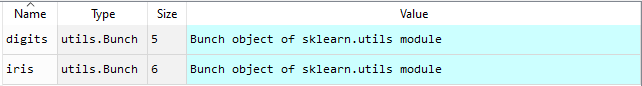
\includegraphics[width=4cm]{figures/1174086/1/variabel.png}
		\centering
		\caption{Isi Variabel Explorer}
	\end{figure}
	\item Mencoba loading an example dataset
	\hfill\break
	\lstinputlisting[firstline=7, lastline=11]{src/1174086/1/1174086.py}
	\item Mencoba Learning dan predicting
	\hfill\break
	\lstinputlisting[firstline=13, lastline=22]{src/1174086/1/1174086.py}
	\item Mencoba Model Persistence
	\hfill\break
	\lstinputlisting[firstline=25, lastline=34]{src/1174086/1/1174086.py}
	\item Mencoba Conventions
	\hfill\break
	\lstinputlisting[firstline=37, lastline=48]{src/1174086/1/1174086.py}
\end{enumerate}

\subsection{Bukti Tidak Plagiat}
\begin{figure}[H]
	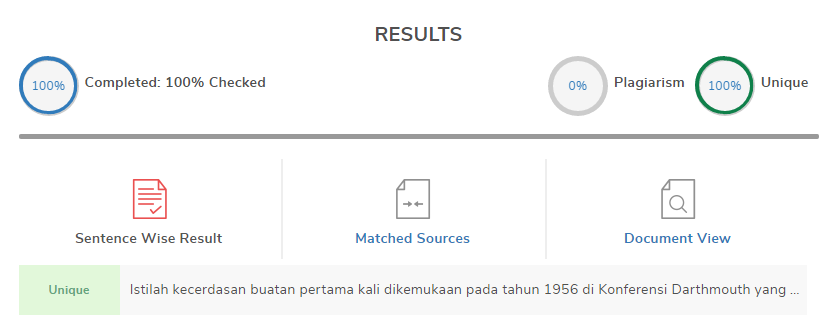
\includegraphics[width=4cm]{figures/1174086/bukti/1.png}
	\centering
	\caption{Bukti Tidak Melakukan Plagiat Chapter 1}
\end{figure}

